\section{Introduction}
\label{sec:intro}

\paragraph{Motivation and goals}
Distributed robotic applications could transform manufacturing, transportation, agriculture, delivery, surveillance, and mapping~\cite{}. Following the trends in cloud, mobile, and machine learning applications, programmability is important in unlocking this potential as robotics platforms become more open and hardware developers shift to the applications marketplace. Available domain specific languages (DSL) for robotics are tightly coupled with platforms, and they combine low-level sensing, communication, and control tasks with the application-level logic (see the related work section~\ref{sec:related} for  more details). This tight-coupling and the attendant lack of abstraction hinders application development on all fronts---  portability, code reuse, and verification and validation (V\&V).



Our goal is to separate the \emph{platform-independent} decision and coordination tasks from \emph{platform-dependent} concerns such as sensing, communication, and low-level control through abstraction. For example, to develop an application for distributed package delivery with mobile robots, the code for waypoint assignment, load-balancing, and handling failures should abstract away detailed implementations of functions for low-level navigation, communication, and control. Applications like these can also be ported across different hardware platforms with the appropriate platform-specific implementations of these abstractions, e.g., steering control subroutine for particular vehicles hardware.
%
In addition, this separation will help combine different analysis techniques that target the platform dependent and independent components respectively. For example, in this paper we show how symbolic executions for the application program can be combined with model-free and data-driven analysis of the platform-specific controllers.\rg{include/exclude based on dryvr analysis.}


\paragraph{Approach} In this paper, we present $\lgname$: a language and supporting verification and testing tools for programming distributed robotic systems. 
\begin{noinditem}
\item {\em For the application developer}, our $\lgname$ language provides key abstractions (\emph{sensor and actuator ports, distributed shared memory, and synchronous execution}) to develop robot applications that interact with the the physical environment, and other participating robot programs.
\item {\em For the V\&V engineer}, the \K-based formal executable semantics we have developed for $\lgname$ and our Z3-based prover, can help discharge key invariants of the $\lgname$ applications (in some cases, automatically) . This verification process also helps identify the {\em platform-dependent\/} proof obligations (or assumptions) that have to be discharged or validated through simulation and testing.
\item {\em For the platform engineers\/} deploying the robot applications, our abstraction makes the $\lgname$ programs portable across platforms, and our high-fidelity $\lgname$ simulator help test the exact same code on different platforms.
\end{noinditem}

\begin{figure}[h!]
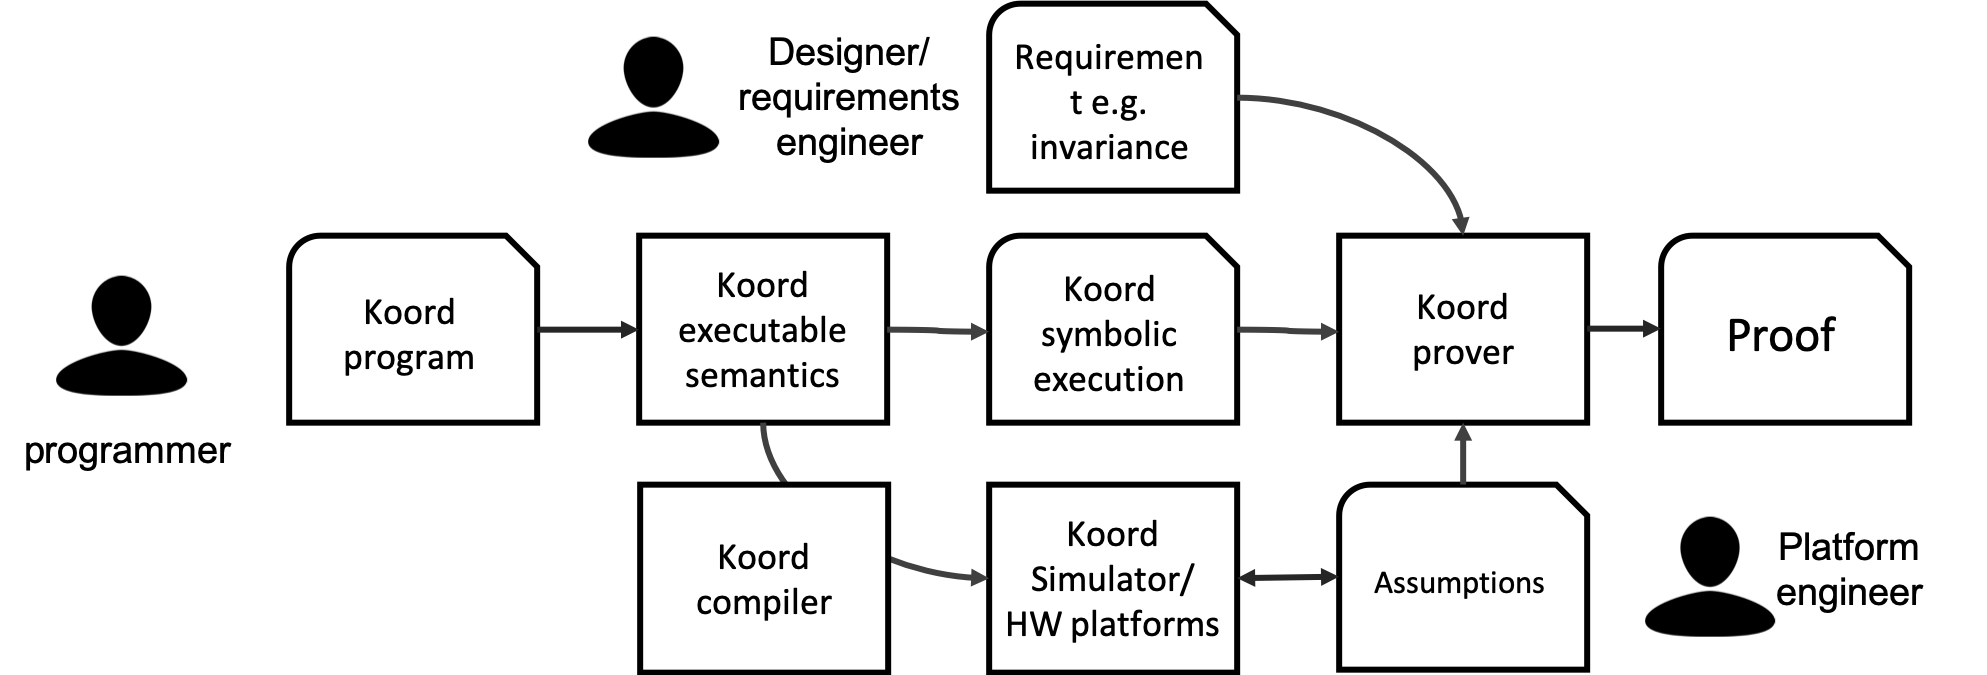
\includegraphics[width=\linewidth]{figs/koorduser.png}
\caption{\small \lgname language  enables programmers to develop distributed robotics applications using a high-level language and prove properties using symbolic executable semantics in \K. Platform specific assumptions are abstracted and can be checked using simulations and hardware deployments.}
\label{fig:koorduser}
\end{figure}

\paragraph{Technical challenges and design decisions}
Formally reasoning about a collection of robots communicating, coordinating, and interacting with a physical environment is complexified by  cyber-physical interactions, concurrency and asynchrony, noise, disturbances, and the lack of precise models for sensors and robot platforms. In managing these complexities, we have baked-in several abstractions in the design of $\lgname$.
%

\begin{noinditem}
\item We introduce an abstract interface of \emph{sensor} and \emph{actuator ports} through which a $\lgname$ program interacts with its environment. The program can read from sensor ports to receive updates about its environment;  and it can write to actuator ports to direct the low-level controllers and actuators. Beyond the names and types of these ports, the abstract interface may specify additional assumptions \sayan{requirements/pre-post conditions} that these ports should satisfy. The $\lgname$ programmer gets to assume these requirements to reason about the $\lgname$ application, while the platform engineer has to ensure that these requirements are indeed met by the implementation of the abstract interface for each platform.


\item We provide a {\em distributed shared memory (DSM)\/} construct for $\lgname$ applications on different robots to communicate with each other. This makes  $\lgname$ applications very succinct (see examples in \reffig{lineform}), and raises the level of abstraction for the programmers beyond sockets, message queues, ROS topics~\cite{}, and the such like. We have developed an implementation of distributed shared memory using UDP messages and \rg{deployed it across different robotic hardware platforms.}
\item Our formal executable semantics of $\lgname$ in the \K framework, assumes a {\em synchronous round-by-round computation model for the distributed system\/}. Each round lasts for a duration of time($\delta >0$) during which both the robots perform discrete computation and interact with the environment. First, each robot executes some {\em event\/} in its program; the different events for different robots may interleave in arbitrary order. Each event may read sensor port values, update program variables and actuator port values, it may send  some messages to update the shared variables. Then, the robots interact with the enviroment (for instance, move according to their set actuator values), updating their sensor ports for the next round. This synchronous model is a restrictive but standard model for distributed computing~\cite{lynch1996a,attiyawelch} and it while it does not completely eliminate concurrency control, it significantly simplifies programming and verification. $\lgname$ provides constructs for mutual exclusion as additional mechanisms for concurrency control with shared variables. This model can be implemented under typical synchrony assumptions for multi-robot networks\footnote{Bounded message delays and clocks with bounded drifts.}.
\item In order to reason about a {\em closed-loop\/} system,  one has to specify or model how the platform-dependent parts of the system react to the actuator values set by the $\lgname$ application. In practice, a detailed model of the platform (e.g., dynamical models for cars, wheel friction, engine torque, etc.) may not be available. Over the past thirty years, the control theory and the hybrid systems communities have developed a bouquet of techniques for reasoning about software-controlled physical processes (dynamical systems) with different types of models~\cite{alurbook, platzerbook,seshiabook}. Our design of the  $\lgname$ semantics is agnostic towards these different approaches. In other words, any available model or actual black-box executable for the platform can be plugged into $\lgname$ semantics, and the corresponding analysis techniques available from the above-mentioned body of work can be brought to bear for verifying the closed system.
\end{noinditem}
These choices do leave out issues related to robot failure,  dynamic joins and leaves, from the current semantics, and could be included in the future. However, even without tackling these issues, $\lgname$ tools can handle analysis of interesting applications and requirements for distributed formation, task allocation, and mapping as demonstrated in \refsect{verification}.

%The program plane consists of a $\lgname$-program executing within the runtime system of every agent. The plant plane consists of the hardware platform of the agent. The control plane acts as a bridge between the program and the plant planes. It receives decisions from the program through the {\em actuator ports\/} (e.g., a sequence of way-points to visit, a temperature to maintain) and drives the plant by making low-level, hardware-dependent decisions (e.g., steering angles, throttle, turning furnaces on or off). It also makes information about the plant's state  (e.g., position coordinates, room temperatures) available to the program through the {\em sensor ports}. This decomposition enables us to formalize the semantics of $\lgname$ with the environment (controller and plant) as a parameter. It also makes it possible to develop verification tools that combine application semantics and environment behavior either as an explicit model, or an executable black-box.


%A $\lgname$ program running on an agent consists of a collection of events specified by preconditions and effects, and it interacts with the environment through sensor and actuator ports. The runtime system executes at most once event every $\delta > 0$ time units, where $\delta$ is a hardware dependent parameter. The preconditions are predicates over (local) program variables, shared variables, and the sensor ports. The effects are statements that update the variables and the actuator ports. 
%
%%
%$\lgname$ has language constructs for facilitating coordination across multiple agents. 
%Shared variables make it straightforward to translate textbook algorithms for consensus, pattern formation, and flocking into code~\cite{Blondel}.
%%
%$\lgname$ supports descriptions of CPS almost as hybrid automata, where event preconditions allow users to specify guards and state invariants using \emph{urgent} and \emph{enabled} preconditions. We discuss this in detail in~\refsect{semantics}.  The distributed nature of these protocols results in nondeterministic behavior, and $\lgname$ captures these behaviors as well. 
%
%We developed the executable semantics of $\lgname$ in the \K framework~\cite{rosu-serbanuta-2013-k}. \K is a rewriting-based executable framework for defining language semantics. Given a syntax and a semantics of a language implemented in \K, a parser, an interpreter, and other support features for formal analysis become available at no additional development cost. 
%
%The design of $\lgname$ aims to reduce the gap between i)~the hybrid automata-driven study of distributed cyber-physical systems and ii)~the feasibility of implementation of the systems. These areas involve related but entirely different hardware level concepts of control and sensing, and software level concepts of distributed protocols and program interactions.%\fTBD{Too long sentence. Please break.}
%
%The semantics of $\lgname$  implemented using the \K semantic framework enables us to construct an executable semantics of the language.
%Our semantics facilitates the development of formal analysis tools using techniques such as symbolic post-state computation and bounded-model-checking combined with sensitivity analysis. We present our tools in \refsect{verification}. To our knowledge, this is the only distributed (CPS) system analysis framework with a language semantics component to it, thus reducing the gap between theory and practice.
%Furthermore, as \reffig{krdarch} shows, the components of the $\lgname$ framework interact using interfaces, allowing interchangeability of formal analysis components. For instance Z3 can be replaced by any other SMT solver depending on the user requirements. In fact, by using \K to implement the executable language semantics, we leave room for consistent extensibility of the language to support even more diverse applications.   
%
%\begin{figure}
%\input{diagram.tex}
%\caption{\scriptsize{$\lgname$ Framework: The front-end generates input program $P$ and candidate invariant $\mathit{inv}$ for the executable semantics in \K. \kbmc\ combines traces generated by the black-box with concrete executions to produce simulation outputs. This in turn provides its \emph{traces} to DryVR to determine whether $\mathit{inv}$ is an $n$-invariant. In \kiic, a symbolic post generation component implemented in \K takes $P$ and $\mathit{inv}$ as input. It outputs constraints that can be processed by a \emph{K-Z3 interface} which is used to check $\mathit{inv}$.}} 
%\label{fig:krdarch}
%\end{figure}

%We implemented a suite of benchmarks and used both our formal analysis tools of inductive invariant verification and bounded model checking to verify them or find counter examples. As expected, the state space expands exponentially with the number of agents due to the inherent non-determinism of distributed CPS captured by our system, which is a factor for the running time of both our approaches. However, inductive invariant checking scales much better than explicit state bounded model checking. We also combined the two approaches to analyze and refine a distributed application with a partially known environment model for an automated \emph{traffic} intersection navigation application. Aside from the theoretical and formal analysis, we performed hardware experiments to confirm the assumptions we made while developing the language semantics for $\lgname$. We assume that \begin{inparaenum}\item each participating agent in a system is known \item time taken to execute a computational step can be considered 0 logical time, or negligible compared to $\delta$, \item shared variable updates propagate to all agents immediately \end{inparaenum}. Our hardware experiments support these assumptions. 


%\paragraph{Incomplete model for environment}
%
%Need explicit language constructs for black-box parts.
%
%Allow trade-off between exposing more low level details and simplicity of the language constructs
%
%For formal analysis, requires specifying assumptions over black-box parts.


\begin{figure}[h!]
\begin{minipage}{0.32\columnwidth}
	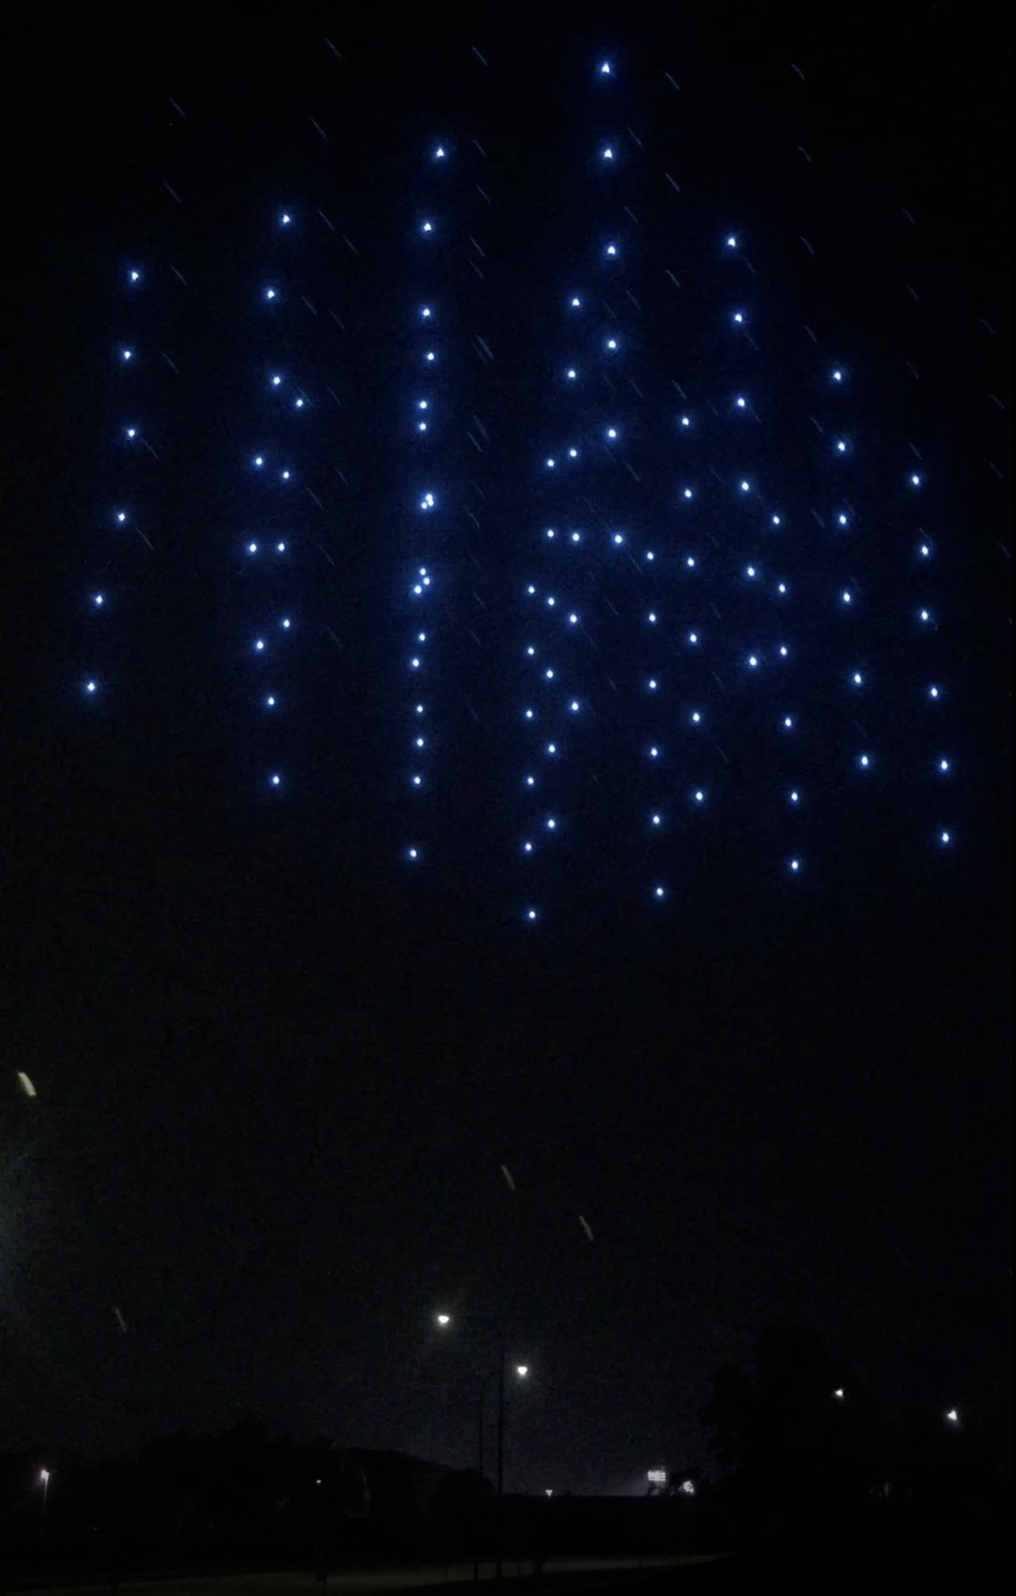
\includegraphics[width=\linewidth]{figs/firefly.png}
\end{minipage}
\begin{minipage}{0.55\columnwidth}
	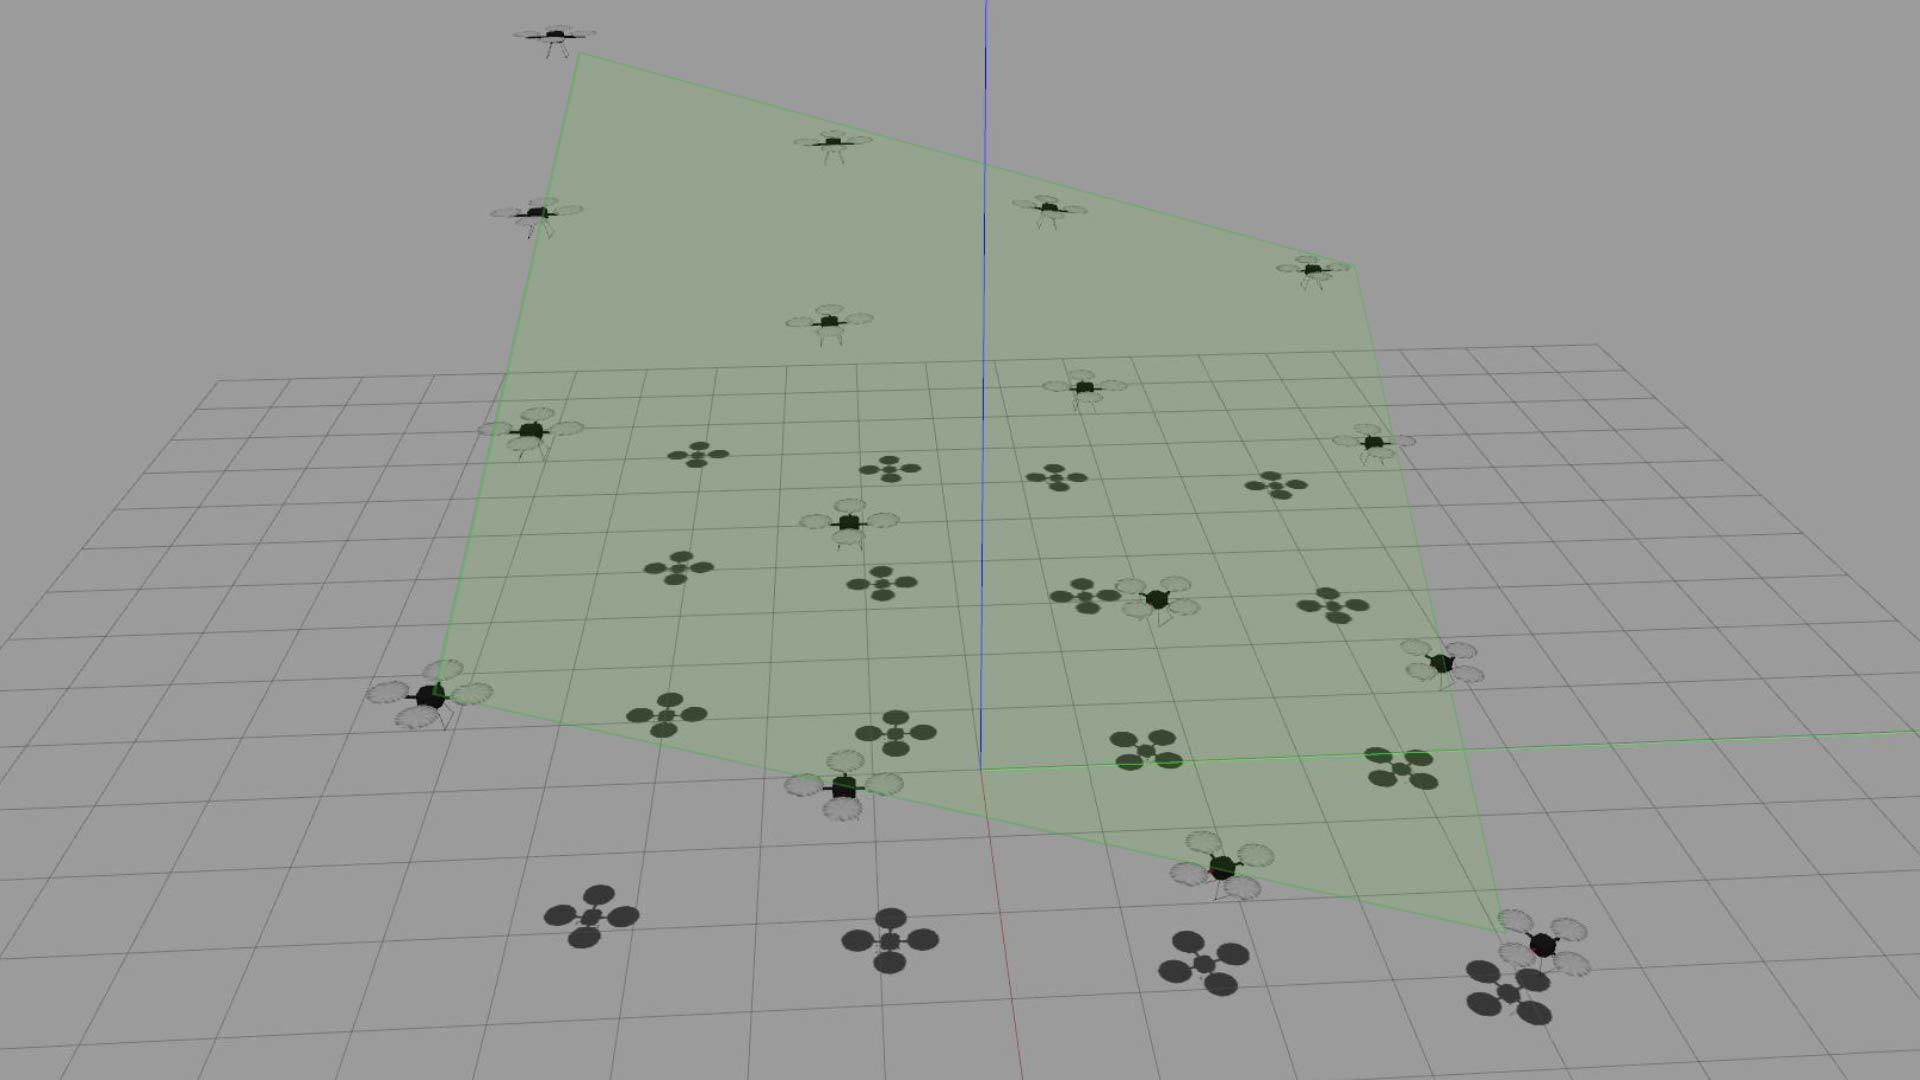
\includegraphics[width=\linewidth]{figs/shapeform_16.jpg}

	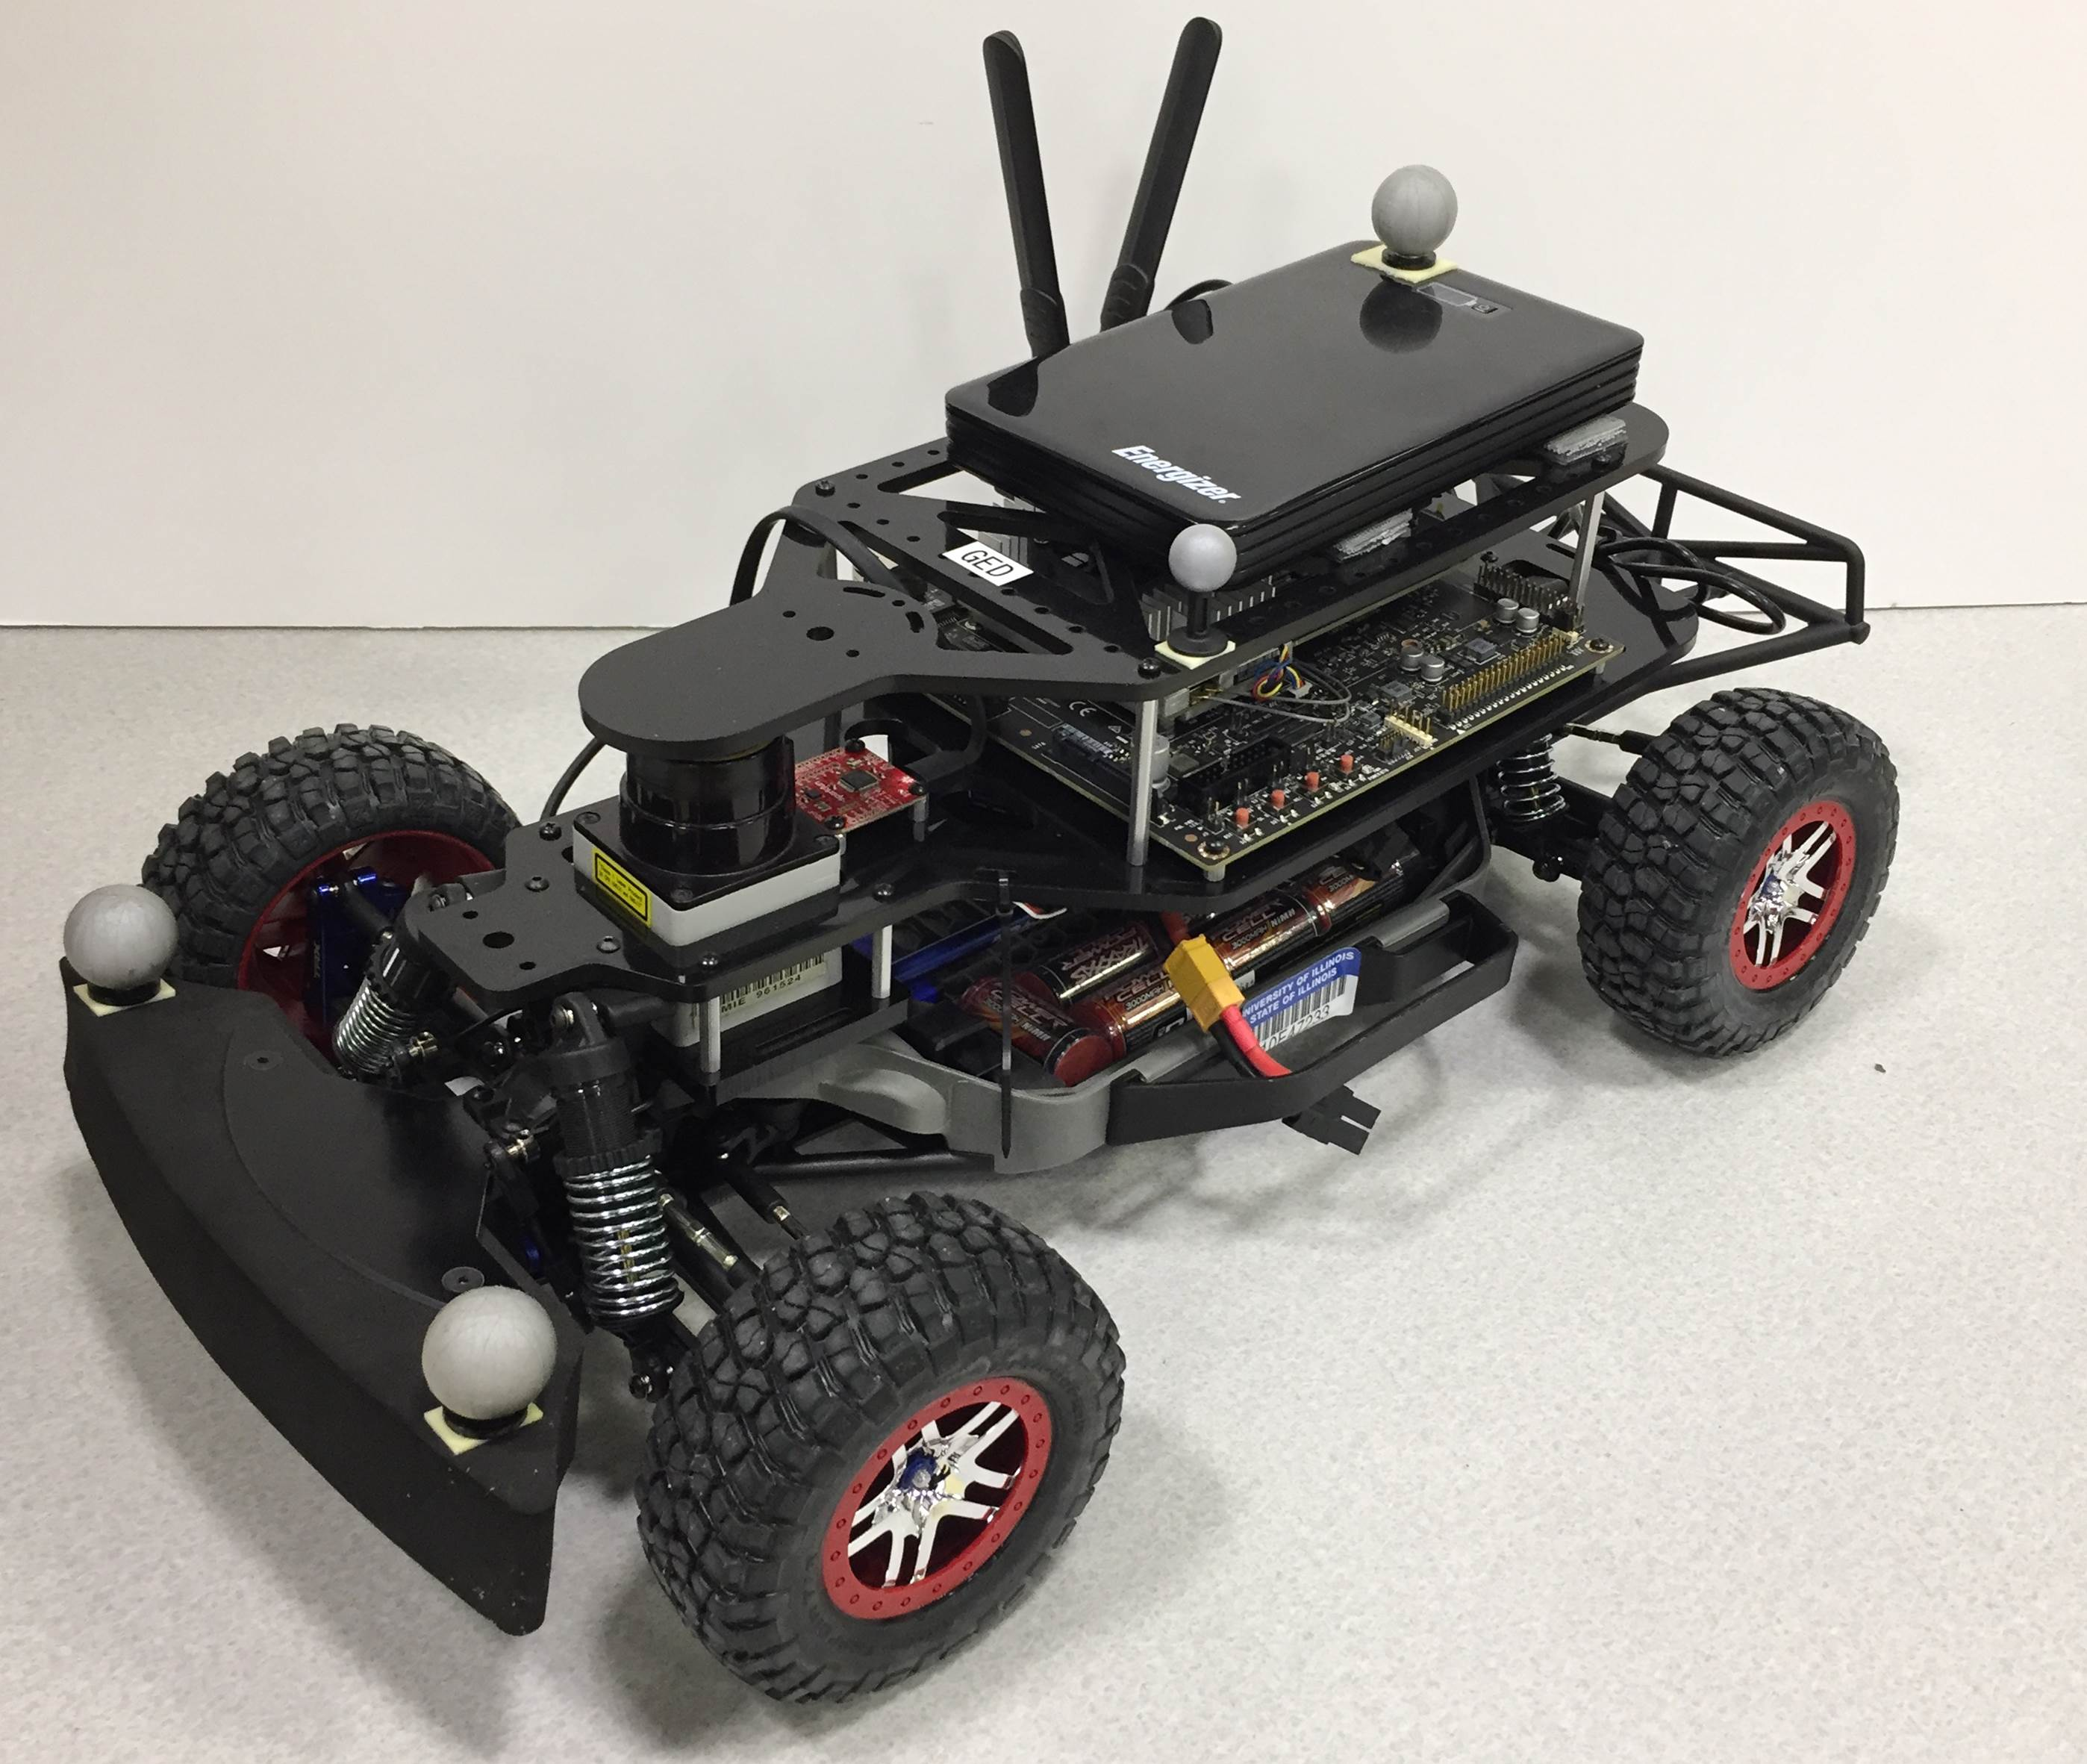
\includegraphics[width=0.42\linewidth]{figs/car.jpg}
	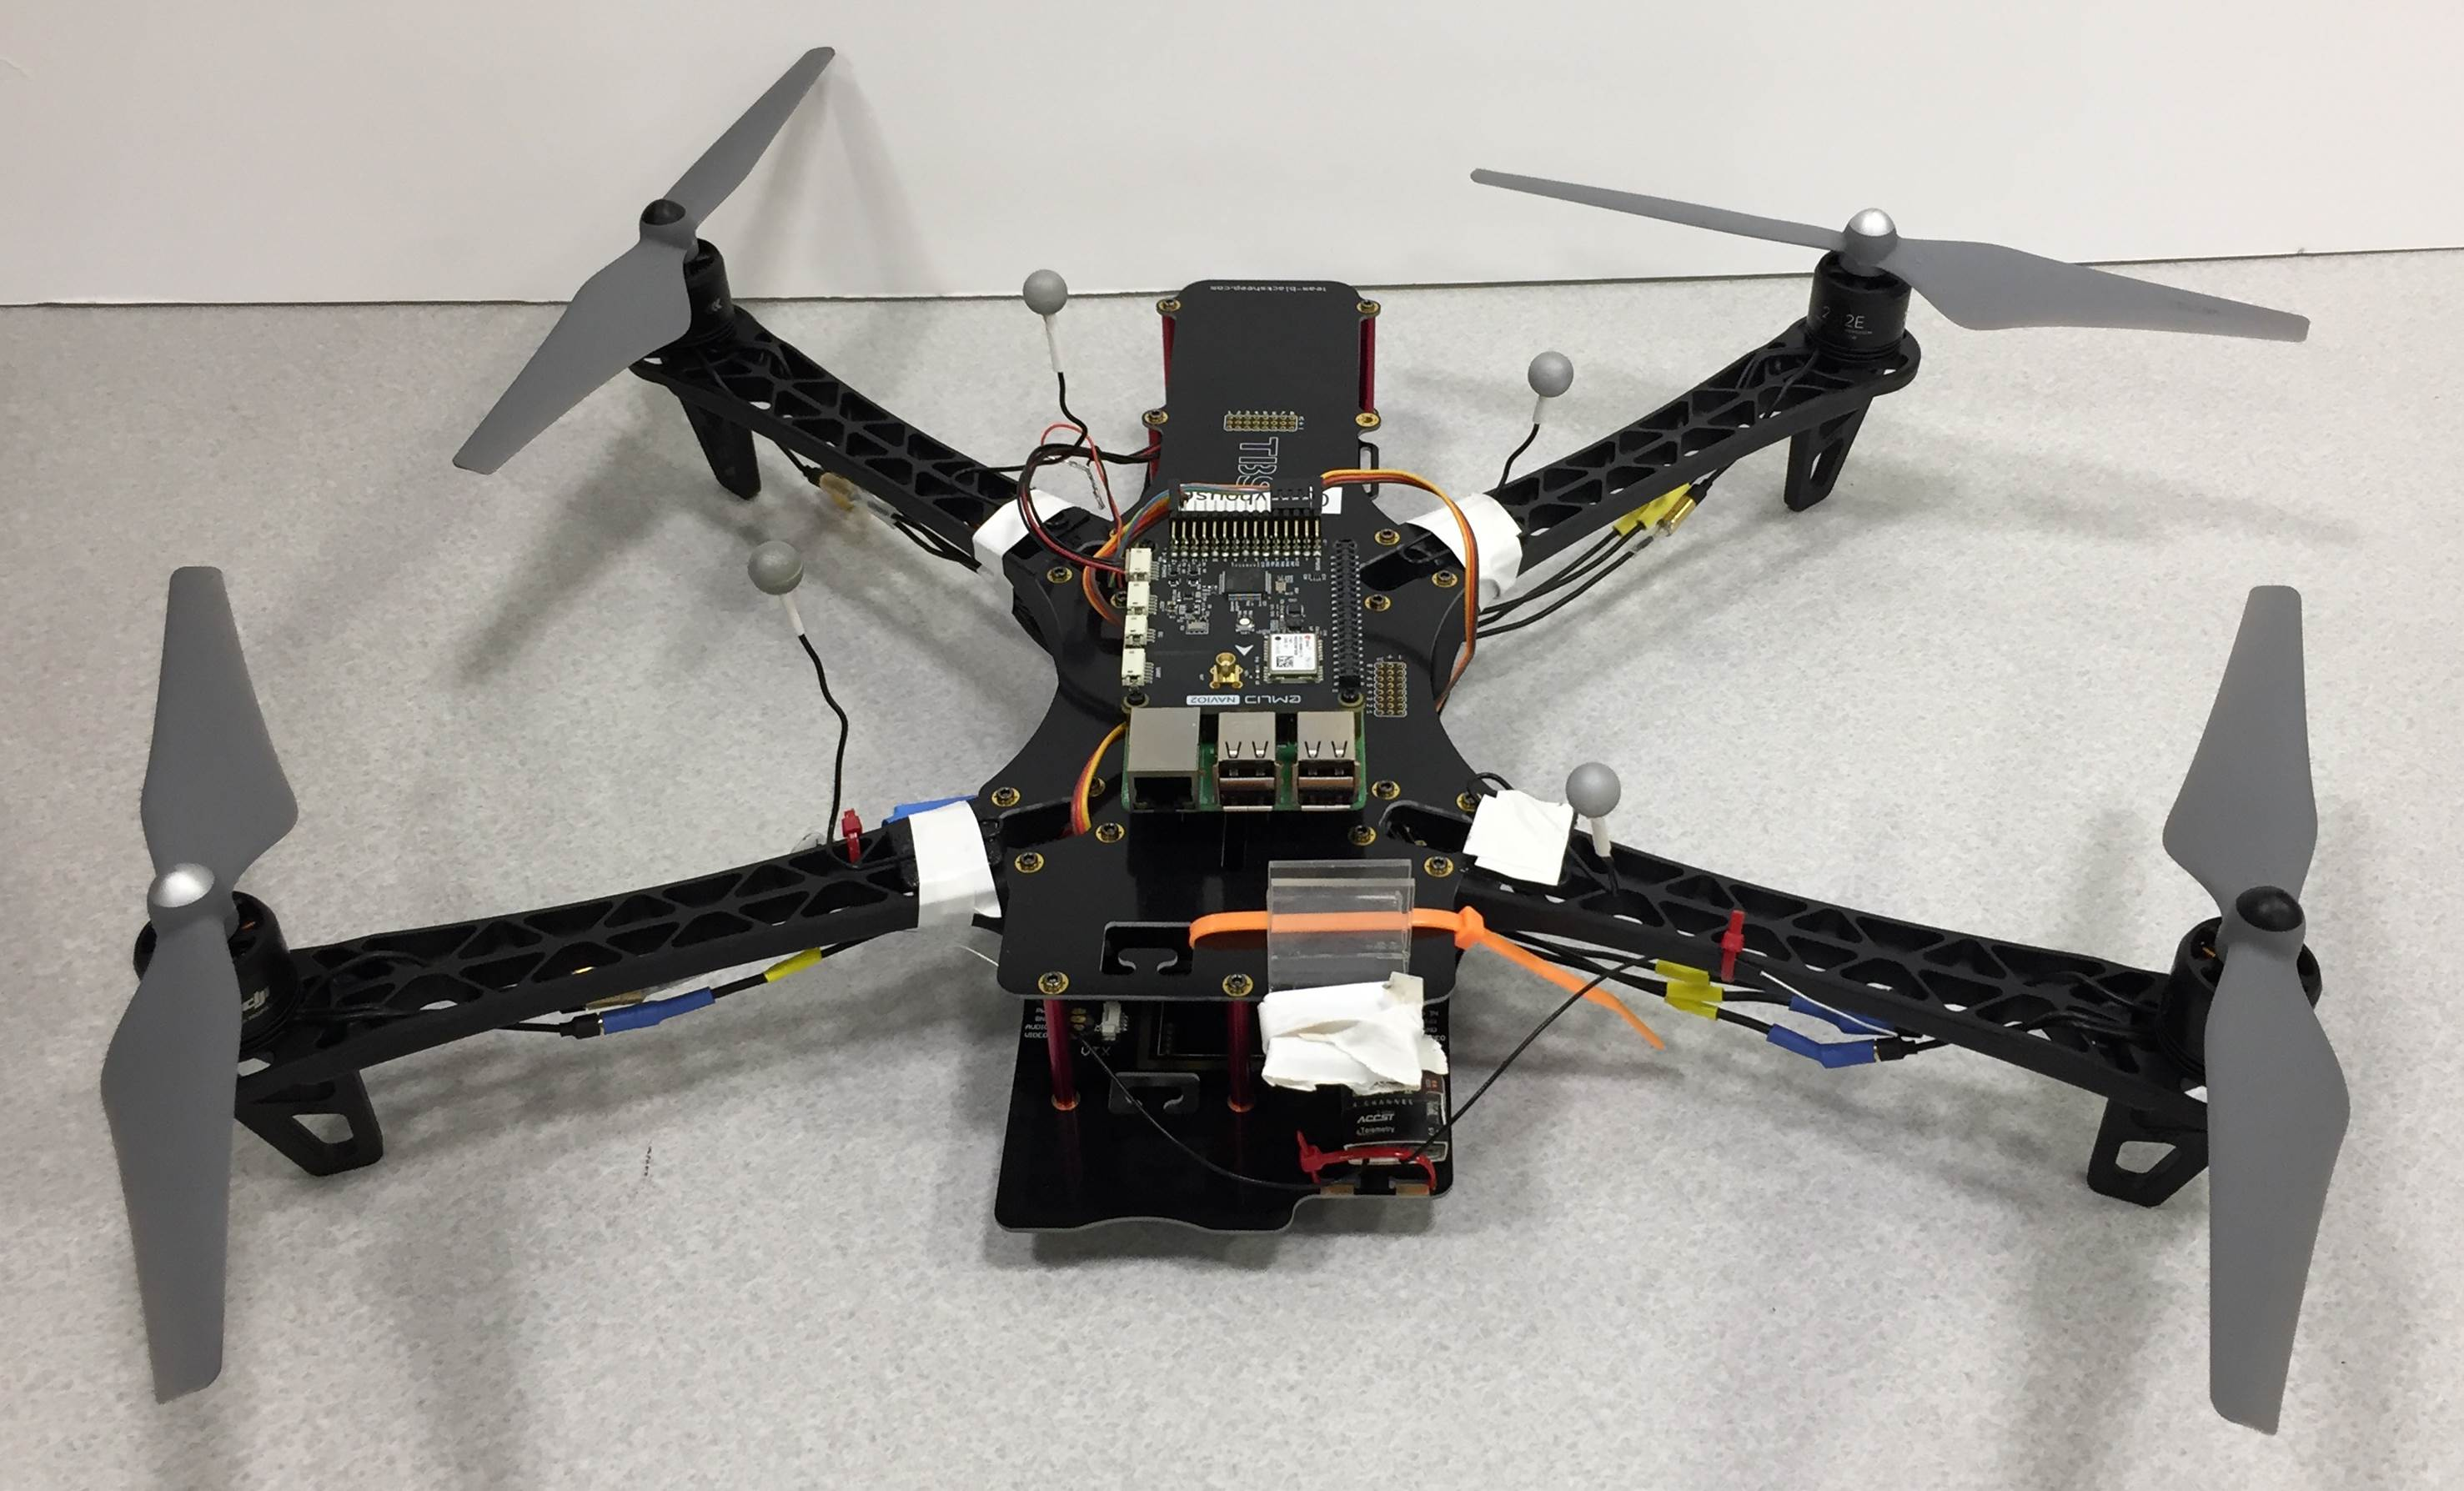
\includegraphics[width=0.56\linewidth]{figs/quad.jpg}
\end{minipage}%
	\caption{Swarm formation show by FireFly Inc. (\emph{Center}). Simulation of shape formation (\emph{Right}).}
    \label{fig:firefly}
\end{figure}

%\paragraph{Implement trusted run-time environment}

%\marginpar{\scriptsize\sayan{[EuroSys'17] An Empirical Study on the Correctness of Formally Verified Distributed Systems.}}
\begin{noinditem}

\item  {We have developed the $\lgname$ language which provides, as first-class constructs,  abstractions for robot  programs to interact with the physical platform, as well as other robot programs.}
\item These abstractions allow $\lgname$ programs to be portable across different hardware;
      we discuss our experiences in deploying several $\lgname$ applications on heterogeneous collections of ground vehicles and drones in Section~\ref{}.
\item  We have developed the formal executable semantics of $\lgname$ using the \K framework. To our knowledge this is the first formalization of a programming language for distributed cyber-physical systems which has also been deployed on actual platforms.
\item  We built analysis tools on top of semantics to facilitate both inductive invariant checking and state space exploration with black-box dynamics. In this paper, we proved inductive invariants for the benchmarks using symbolic execution while identifying assumptions and proof obligations. While most formal analysis tools for distributed systems verify models of the protocols in form of automata, this framework actually verifies the program implementing the abstract model.
\item An intended useful outcome of this methodology is a list of formal assumptions for the platform or implementation specific components such sensors, schedulers, data structures, etc. In the end-to-end safety assurance cases~\cite{} for complex cyber-physical systems, these assumptions can serve as contracts for sensing devices, drivers, hardware platforms, and operating system modules that are often outside the control of the application programmer.
\item Our design of \lgname creates a separation of device-specific from device-independent concerns. In our implementation, we enforced simple interface for every device-specific sensor and actuator modules. These interfaces allow a user to deploy (and simulate) the same program on heterogenous devices using \emph{configurations} without any alteration to the $\lgname$ program, or any additional compilation, thus shortening the test-debug-deployment cycle.
\item We explored the trade-off between the level of abstraction of the minutiae of multi-robot systems and achieved a simple yet expressive language design enabling a versatile set of multi-robot applications. One of the design choices we made was to abstract away continuous time in language. This required a careful design of the memory model to provide consistency and sychrony guarantees. We achieved distributed shared memory through round-based synchronous message passing. Our compiler translates $\lgname$ programs to Python and a device-independent middle-ware implements the memory model and module interfaces.
\item We created a simulation environment in Gazebo for testing $\lgname$ applications and validating assumptions, specifically on robot-environment behavior. The simulation environment only differs from a hardware deployment environment in the dynamics models of the physical platforms, but all software components are identical.

\rg{Not sure how to phrase these}
%\item Enable (manual) formal analysis (for example, on DMap or Task)
\item Convert pub-sub based message passing to black-box module interface
\item Wrap around black-box modules (ROS packages) to satisfy assumptions identified in formal analysis : Most technically challenging but difficult to sell

%\item Finally, \sayan{experimental evaluation. What did we learn that can generalize beyond this specific application? How did we extend CyPhyHouse capabilities generally?}

\end{noinditem}
%\makeatletter
%\let\origsection\section
%\renewcommand\section{\@ifstar{\starsection}{\nostarsection}}
%
%\newcommand\nostarsection[1]
%{\sectionprelude\origsection{#1}\sectionpostlude}
%
%\newcommand\starsection[1]
%{\sectionprelude\origsection*{#1}\sectionpostlude}
%
%\newcommand\sectionprelude{%
%  \vspace{-0.5em}
%}
%
%\newcommand\sectionpostlude{%
%  \vspace{0em}
%}
%\makeatother
%The application program \dmap is X lines of \lgname code with a \sayan{handful} external functions.
%%
%The application program, takes full advantage of the \lgname language's features shared memory semantics.
%Individual robots update their local maps using LIDAR scans, and a \sayan{single line of \lgname code} merges the local maps to update the shared global map.
%\sayan{Similar sentence about path planning and sensing.}
%
%
%Second, the modular structure and semantics of the \dmap application makes it possible to formally reason about its correctness. We illustrate this by proving key correctness and consistency properties of the application, namely that, \sayan{write informally.}
%%
%


%The simulator enables the user to test their discrete event loop with simple motion models to test and debug the application program logic without incurring the cost of hardware deployment in case of buggy programs.
%The simulator also serves as a visualization tool as it can be used to plot the behavior of any program variables, or controller variables. For instance, we implemented a robot \emph{formation} app in $\lgname$, where several robots form a shape in which they are evenly distributed.

%\subsubsection{Other by-products}


%Design and development of the CyPhyHouse open source software system. This includes a discrete event simulator for distributed robotic systems, the application launcher, the run-time logging and monitoring system, and an integrated indoor positioning system. All of these software tools are integrated with our new robot programming language called $\lgname$ and its compiler.





%Design and development of the Koord programming language and the supporting verification tool KoordBMC~\cite{koordreport}--- significant, related but separate efforts---are not contributions of the current paper; we discuss their usage for the sake of completeness.
% completely describing the framework.
% the Demonstration of an example application development using CyPhyHouse tools and deployment on a physical system using multiple quadcopters.
%Non-contributions: Spell these out  to avoid misdirected criticisms and conflict with overlapping publications.
%\begin{itemize}
%\item Language design
%\item Verification tools.
%\item Low-level controller design for vehicles.
%\end{itemize}

%\begin{figure}[h!]
%\centering
%\includegraphics[width=0.45\textwidth]{figs/exp_traces.png}
%\caption{\small Experimental run in our testbed. The traces show the path of each robot for the last $2$ seconds. }
%\label{fig:exp_traces}
%\end{figure}


